\documentclass[a4paper,11pt]{article}

\usepackage[utf8]{inputenc}

\usepackage{graphicx}
\usepackage{caption}
\usepackage{subcaption}

\usepackage{pgfplots}
\pgfplotsset{compat=1.18} 

\usepackage{minted}

\begin{document}

\title{
    \textbf{Searching}
}
\author{Edward Sharp}
\date{31-01-25}

\maketitle

\section*{Introduction}

\section*{Unsorted Search}

\begin{figure}[h!]
  \centering
  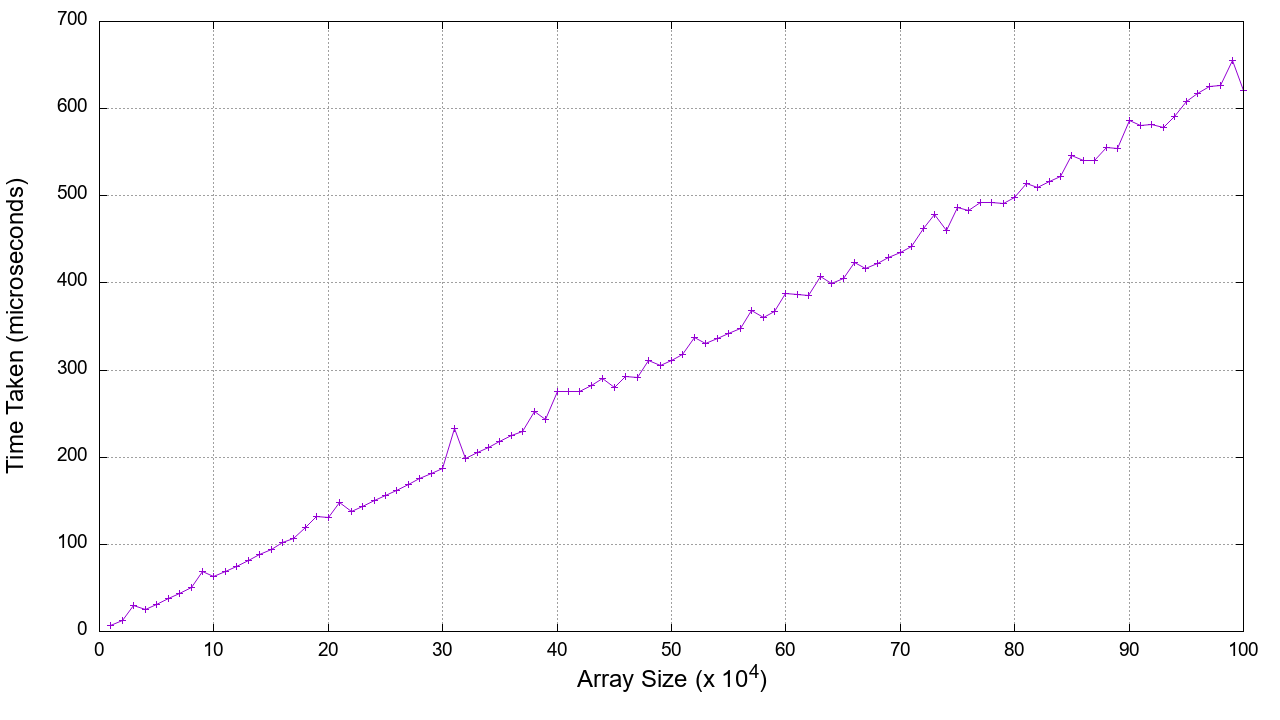
\includegraphics[width=0.8\textwidth]{unsorted_search_plot}
  \caption{Unsorted search, array size plotted against time}
  \label{fig:unsorted_search_plot}
\end{figure}

\section*{Sorted Search}

\begin{figure}[h!]
  \centering
  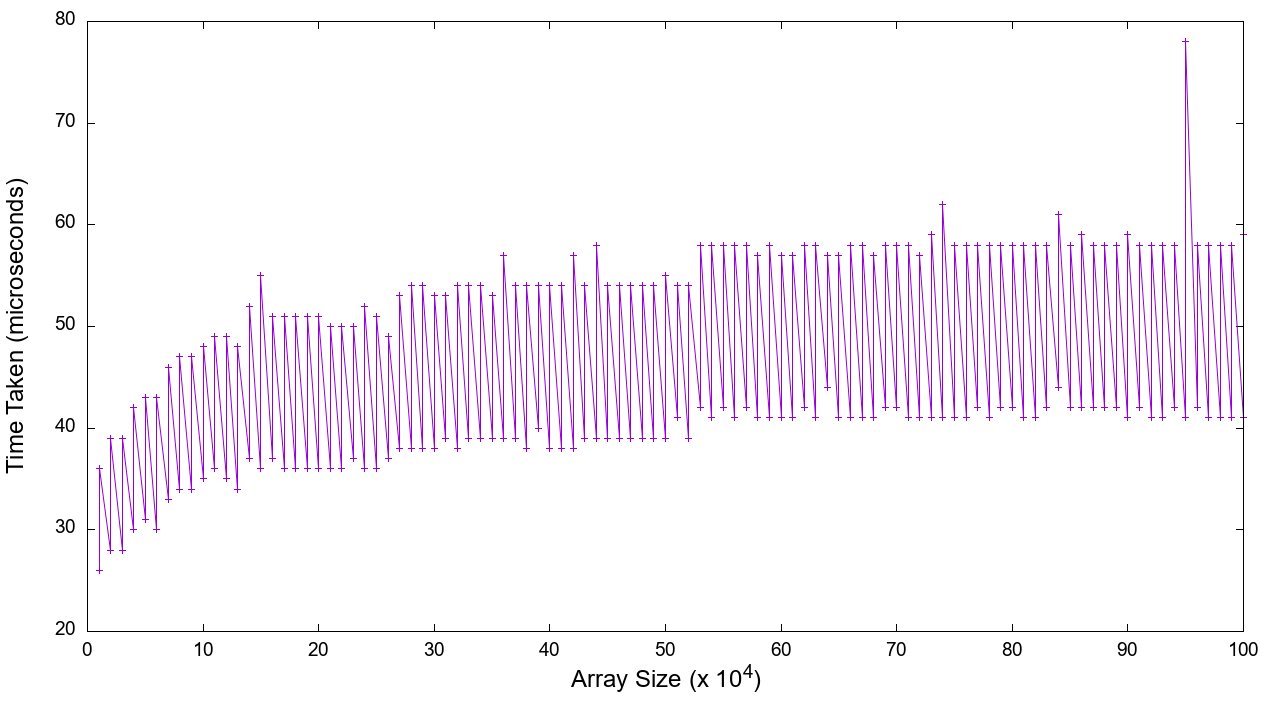
\includegraphics[width=0.8\textwidth]{sorted_search_plot}
  \caption{Sorted search, array size plotted against time}
  \label{fig:sorted_search_plot}
\end{figure}

\section*{Layout}

\subsection{sections}

{\tt *} (for
example {\tt \textbackslash section* }).

\subsection*{inserting code}

{\tt minted}: {\tt List.sort()}.

\begin{minted}{java}
  for (int i = 0; i < 100; i++){
    sum += i;
  }
\end{minted}

\section*{numbers}

$1.2345678 s$ \\
$1.235 s$ or $1.2 s$?

\subsection*{tables}

\begin{table}[h]
\begin{center}
\begin{tabular}{l|c|c}
\textbf{prgm} & \textbf{runtime} & \textbf{ratio}\\
\hline
  dummy      &  115 &     1.0\\
  union      &  535 &     4.6\\
  tailr      &  420 &     3.6\\
\end{tabular}
\caption{Union and friends, list of 50000 elements, runtime in microseconds}
\label{tab:table1}
\end{center}
\end{table}

\section*{no f*ing screen shots}

\section*{graphs}

\begin{figure}[h]
  \centering
  \begin{subfigure}{.5\textwidth}
    \centering
    \includegraphics[scale=0.45]{fib.png}
    \caption{using raster graphics}
  \end{subfigure}%
  \begin{subfigure}{.5\textwidth}
    \centering
    \includegraphics[scale=0.45]{fib.pdf}
    \caption{using vector graphics.}
  \end{subfigure}
  \caption{Difference in image formats.}
  \label{fig:images}
\end{figure}

\begin{figure}
  \centering
  \begin{tikzpicture}
    \begin{axis}[
      xmin=12, xmax=28, ymin=0, ymax=3500,
      xlabel=n, ylabel={time in $\mu s$},
      width=8cm, height=6cm]
      \addlegendentry{runtime fib(n)};
      \addplot[] table {fib.dat};
    \end{axis}

  \end{tikzpicture}
  \caption{The same graph using TikZ}
  \label{fig:tikz}
\end{figure}

The graph in Fig.\ref{fig:tikz} is generated using Tikz and as you can
see, I know have the time in "$\mu s$" instead of in "us".


\section*{\LaTeX things}

Some \LaTeX errors that I frequently see that could easily be avoided
if you only know where they come from.

\section*{less than}

If you in your LaTeX code write "5 \textless\ 7" it will look like 5 <
7 and "9 \textgreater\ 7" will look like 9 > 7. Using the characters
\textless\ and \textgreater\ directly does not work ... so, how did I
do it?  I used the commands {\tt  \textbackslash textless} and {\tt
  \textbackslash textgreater} to generate the symbols \textless\ and
\textgreater.

You could also use {\tt \{\textbackslash tt 5 < 7\}} but then it
will use the teletype font and look like this: {\tt 5 < 7}.

Still another way is to write it using so called {\tt math mode}. This
is a mode used for writing mathematical formulas in a nice way. You
enclose your expression in {\tt \$} signs like this {\tt \$5 < 7\$}
and then it will look like this $5 < 7$.

If you have a larger mathematical expression you enclose it in double
\$ and the result is that it is written centered with some space
around it like this:  $$ 5 < (3 * 8 / 3 ) $$

\subsection{math mode}

There are several ways that you can write $n \log(n)$ in \LaTeX.

\begin{itemize}
\item {\tt \$n log(n)\$}  : which is interprated as $n xyz(n)$ i.e. $n \times l \times o \times g \times (n)$ and since we then omitt the multiplications it will be displayed as $n log(n)$

\item {\tt \$n \textbackslash times log(n)\$} : which is better since
  we then explicitly have one multiplication and it is displayed as
  $n \times log(n)$.

\item {\tt \$n \textbackslash log(n)\$} : which is how it should be
  done, its now displayed as $n \log(n)$.
\end{itemize}  



\subsection*{why strange font}

If you want to write {\em foo} in teletype font you write like this
\verb+{\tt foo}+. If you forget the closing \} then it will look like
this: {\tt foo. Now everything here after until the end of you report
  will look like this. }



\section*{make}





\end{document}
